% arara: pdflatex: { shell: yes }
\documentclass[twoside]{article}
\usepackage[utf8]{inputenc}
\usepackage[english]{babel}
\usepackage{amsmath, amssymb, amsthm}
\usepackage{hyperref}
\usepackage{ragged2e}
\usepackage{graphicx}
\usepackage{float}
\usepackage{fancyhdr}
\usepackage{geometry}
\usepackage{multicol}
\usepackage{url}
\usepackage{listings} % for better code formatting
\usepackage{xcolor} % for syntax highlighting

% suppress underfull and overfull warnings
\tolerance=1000
\emergencystretch=10pt

\setlength{\headheight}{15.2pt}
\geometry{paperwidth=8.5in, paperheight=11.0in, top=1.0in, bottom=1.0in, left=1.0in, right=1.0in}

\pagestyle{fancyplain}
\fancyhead[lo]{Activity \#4.2}
\fancyhead[co]{}
\fancyhead[ro]{P25-LIS-3012}
\fancyfoot[lo]{\thepage}
\fancyfoot[co]{Advanced Databases, UDLAP}
\fancyfoot[ro]{}

\begin{document}

\fancypagestyle{plain}{
  \renewcommand{\headrulewidth}{1pt}
  \renewcommand{\footrulewidth}{1pt}
}

\title{Design of a Distributed Database}
\author{\small{Erick Gonzalez Parada ID: 178145}\\
  \small{Emiliano Ruiz Plancarte ID: 177478} \\
  \small{Andre Francois Duhamel Gutierrez ID: 177315} \\
\small{Antonio Gutiérrez Blanco ID: 177442}}
\date{\today}
\maketitle

\begin{abstract}
  \raggedright
  This document explores the practical design of a distributed database for managing multimedia content related to movies and music. The design includes a conceptual schema (UML), a relational schema, and a query interface for interacting with the database. We implement a Java CRUD application that demonstrates vertical fragmentation in CockroachDB, a distributed SQL database system.
\end{abstract}

\begin{justify}
  \textbf{\textit{Keywords:}} Multimedia, Database Design, Distributed Database, UML, Query Interface, Vertical Fragmentation, CockroachDB.
\end{justify}

\section{Objective}
The objective of this exercise is to develop practical skills in database design by analyzing a given scenario and proposing a database solution. This includes designing the conceptual schema (UML), the relational schema, and a query interface for interacting with the database. Additionally, we implement a practical Java application that demonstrates vertical fragmentation in a distributed database environment using CockroachDB.

\section{Theoretical Framework}

Distributed database systems represent a paradigm shift from traditional centralized databases by distributing data across multiple geographic locations while maintaining a unified logical view for users \cite{geekforgeeks}. These systems offer several advantages including improved performance, reliability, and availability.

\subsection{Types of Data Distribution}

There are two primary approaches to distributing data in a distributed database system:

\begin{itemize}
  \item \textbf{Horizontal Fragmentation (Sharding):} Divides tables by rows across different locations. Each location contains a subset of the complete data set but maintains the same schema structure \cite{mongodb}.
  
  \item \textbf{Vertical Fragmentation:} Divides tables by columns across different locations. Each location contains specific attributes of the data, which can be optimized based on access patterns or regional requirements \cite{cockroachlabs}.
\end{itemize}

Our implementation focuses on vertical fragmentation, where different attributes of the movie data are stored in different regions, optimizing data locality and access patterns.

\begin{figure}[H]
  \centering
  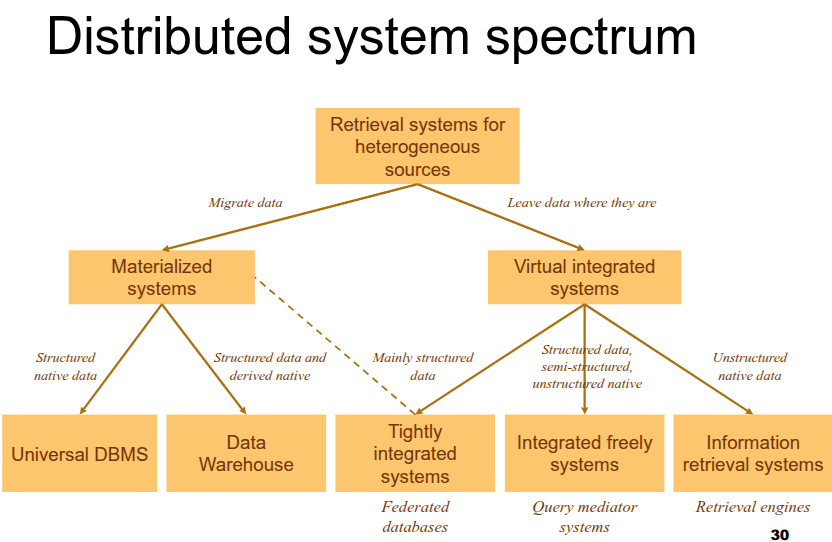
\includegraphics[width=0.5\textwidth]{imgs/distribuitedspectrum.png}
  \caption{Distributed Database Spectrum}
  \label{fig:1}
\end{figure}

\subsection{CockroachDB and Distributed SQL}

CockroachDB is a distributed SQL database that automatically replicates and distributes data across multiple nodes while maintaining ACID compliance \cite{cockroachlabs}. It uses a technique called "multi-active availability" to ensure data consistency across distributed nodes. Key features include:

\begin{itemize}
  \item Automatic sharding and rebalancing
  \item Distributed transactions with serializable isolation
  \item Multi-region deployment capabilities
  \item Survivability during network partitions and node failures
  \item SQL compatibility with PostgreSQL
\end{itemize}

In our implementation, we leverage CockroachDB's multi-region capabilities to demonstrate vertical fragmentation by region, where different attributes of our movie data are stored in different geographic regions.

\section{Summary of the Mini-World Description}
Based on the description of the mini-world from the previous activity, we identified the following main entities:

  
- \textbf{Movie:} Title, duration, release date, classification, directors, producers, actors, and associated soundtracks.
  
- \textbf{Director:} Personal information + filmography.
  
- \textbf{Actor:} Personal information + filmography.
  
- \textbf{Producer:} Name, contact information, list of produced movies, and invested amount.
  
- \textbf{Soundtrack:} Title, author, performers, duration, date, classification.
  
- \textbf{Author:} Personal information + list of written soundtracks.
  
- \textbf{Performer:} Personal information + list of performed soundtracks.
  
- \textbf{Cinephile:} Personal information, favorite music, and favorite movies.


The MyCineMusic database is designed to manage multimedia content, particularly movies and music. It stores information about artists, albums, songs, movies, genres, user ratings, and playback history. To better understand the structure of the mini-world, a UML diagram was created, showing the different classes with their relationships and attributes.

\begin{figure}[H]
  \centering
  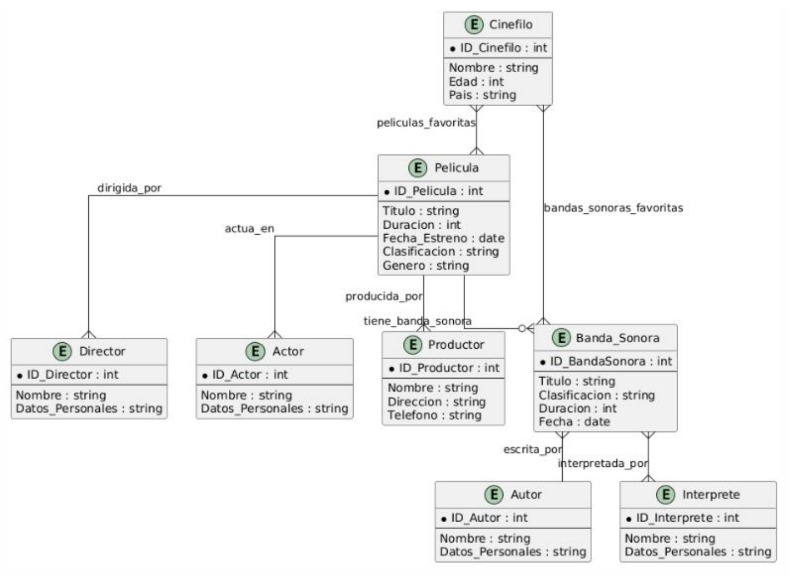
\includegraphics[width=1\textwidth]{imgs/uml.jpeg}
  \caption{UML Diagram of the MyCineMusic Database}
  \label{fig:2}
\end{figure}

\section{Query Space and Interface}

Our implementation consists of a Java CRUD (Create, Read, Update, Delete) terminal application that interacts with a CockroachDB distributed database. This application demonstrates how vertical fragmentation works in a practical distributed database environment.

\subsection{System Architecture}

The application follows a three-tier architecture:

\begin{itemize}
  \item \textbf{Presentation Layer:} A console-based user interface (ConsoleUI class) that handles user input and displays results.
  \item \textbf{Business Logic Layer:} Manages the application logic and data transformations (Movie class).
  \item \textbf{Data Access Layer:} Handles database connections and operations (DatabaseManager class).
\end{itemize}

\subsection{Vertical Fragmentation Implementation}

Our implementation achieves vertical fragmentation through CockroachDB's multi-region capabilities. The \texttt{pelicula} table is partitioned by the \texttt{region} column, which means that different parts of the movie data are physically stored in different geographic regions based on the region value.

\begin{lstlisting}[language=SQL, caption=Table Schema with Region-Based Partitioning]
CREATE TABLE pelicula (
  id UUID PRIMARY KEY DEFAULT gen_random_uuid(),
  titulo STRING NOT NULL,
  duracion INTERVAL,
  fecha_estreno DATE,
  clasificacion STRING,
  region public.crdb_internal_region NOT NULL,
  created_at TIMESTAMP DEFAULT now()
);
\end{lstlisting}

The \texttt{region} column uses the special \texttt{public.crdb\_internal\_region} type, which CockroachDB uses to determine where to physically store the data. When a new movie record is created, the application assigns it to a specific region, and CockroachDB ensures that the data is stored in the corresponding geographic location.

This approach offers several advantages:
\begin{itemize}
  \item \textbf{Data Locality:} Data is stored closer to where it's most frequently accessed, reducing latency.
  \item \textbf{Regulatory Compliance:} Certain data can be kept within specific geographic regions to comply with data sovereignty regulations.
  \item \textbf{Fault Tolerance:} The system remains operational even if one region experiences an outage.
\end{itemize}

\begin{figure}[H]
  \centering
  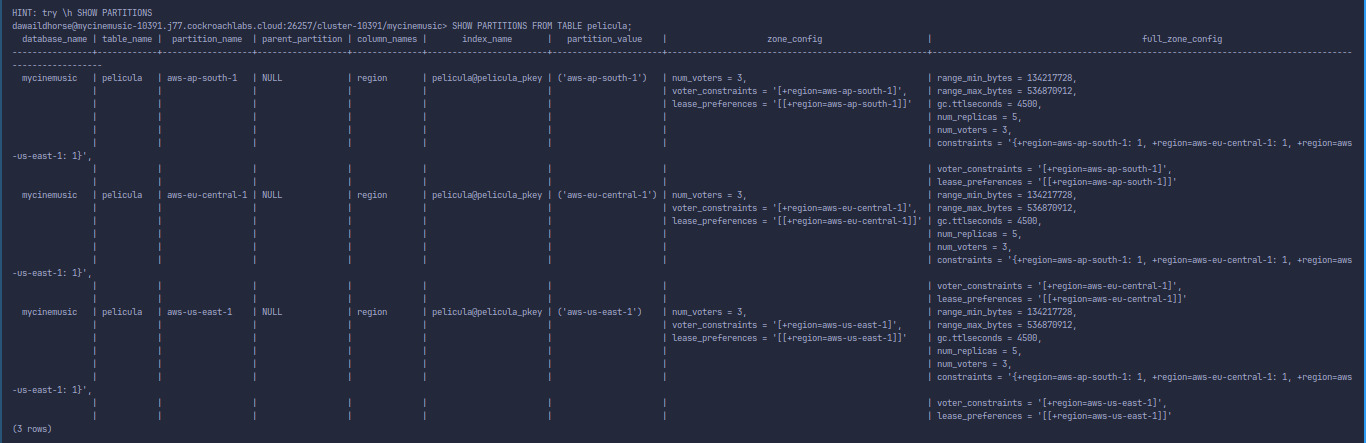
\includegraphics[width=1\textwidth]{imgs/cli.jpeg}
  \caption{Fragmentation observed in CockrouchDB CLI}
  \label{fig:3}
\end{figure}

\subsection{Query Interface}

Our Java application provides a terminal-based interface for interacting with the distributed database. The interface offers the following operations:

\begin{enumerate}
  \item \textbf{Add a new movie:} Creates a new movie record with title, duration, release date, classification, and region.
  \item \textbf{View all movies:} Displays all movies stored in the database across all regions.
  \item \textbf{View movie by ID:} Retrieves and displays a specific movie by its UUID.
  \item \textbf{Update a movie:} Modifies the details of an existing movie.
  \item \textbf{Delete a movie:} Removes a movie from the database.
  \item \textbf{Show database partitions:} Displays information about how the data is partitioned across regions, demonstrating the vertical fragmentation.
  \item \textbf{Check database connection:} Verifies the connection to the CockroachDB cluster.
\end{enumerate}

\subsection{Demonstrating Vertical Fragmentation}

The application includes a special feature to visualize the vertical fragmentation through the "Show database partitions" option. This executes the \texttt{SHOW PARTITIONS FROM TABLE pelicula} command, which returns information about how the data is distributed across different regions.

The output shows that different rows are physically stored in different regions based on the \texttt{region} value, demonstrating vertical fragmentation in action. This approach allows for region-specific optimizations and ensures that data is stored close to where it's most frequently accessed.

\section{Implementation in Java}

\begin{figure}[H]
  \centering
  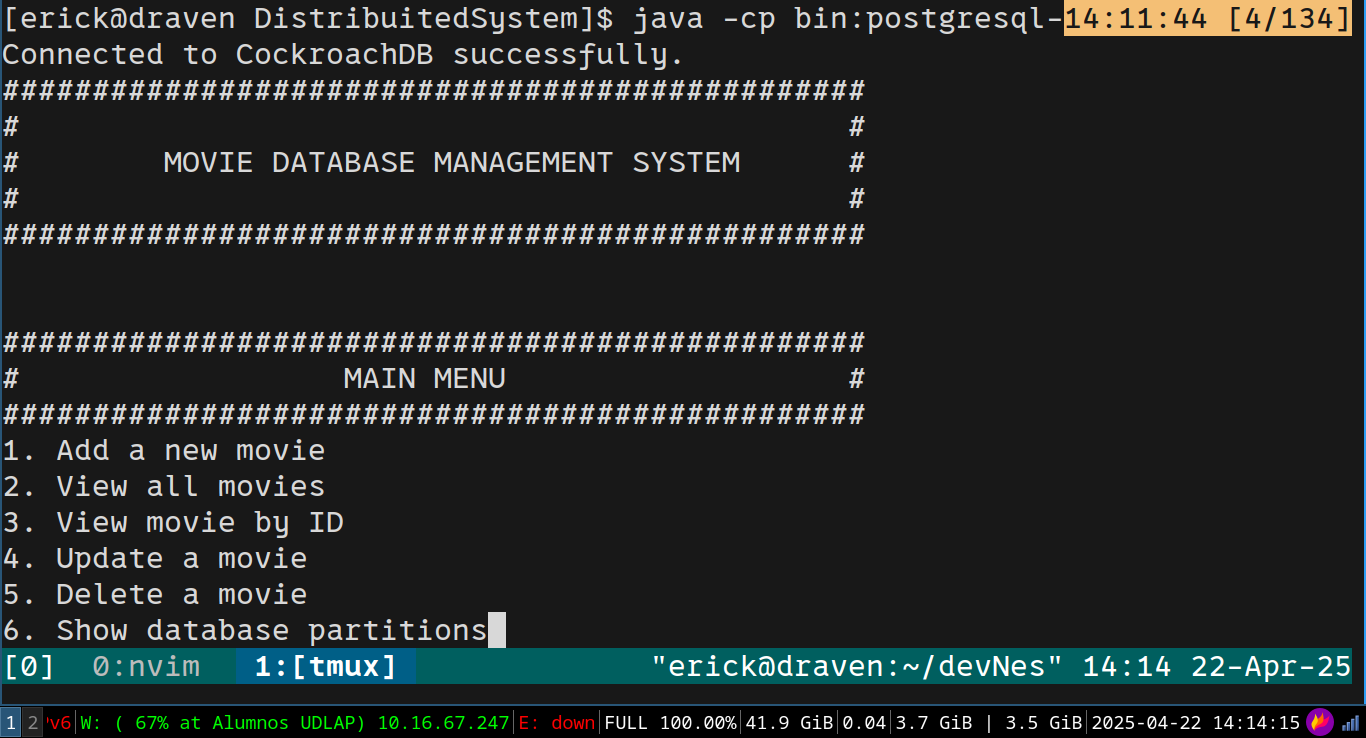
\includegraphics[width=1\textwidth]{imgs/jav1.png}
  \caption{Java Implementation of the MyCineMusic Database, menu}
  \label{fig:4}
\end{figure}


\begin{figure}[H]
  \centering
  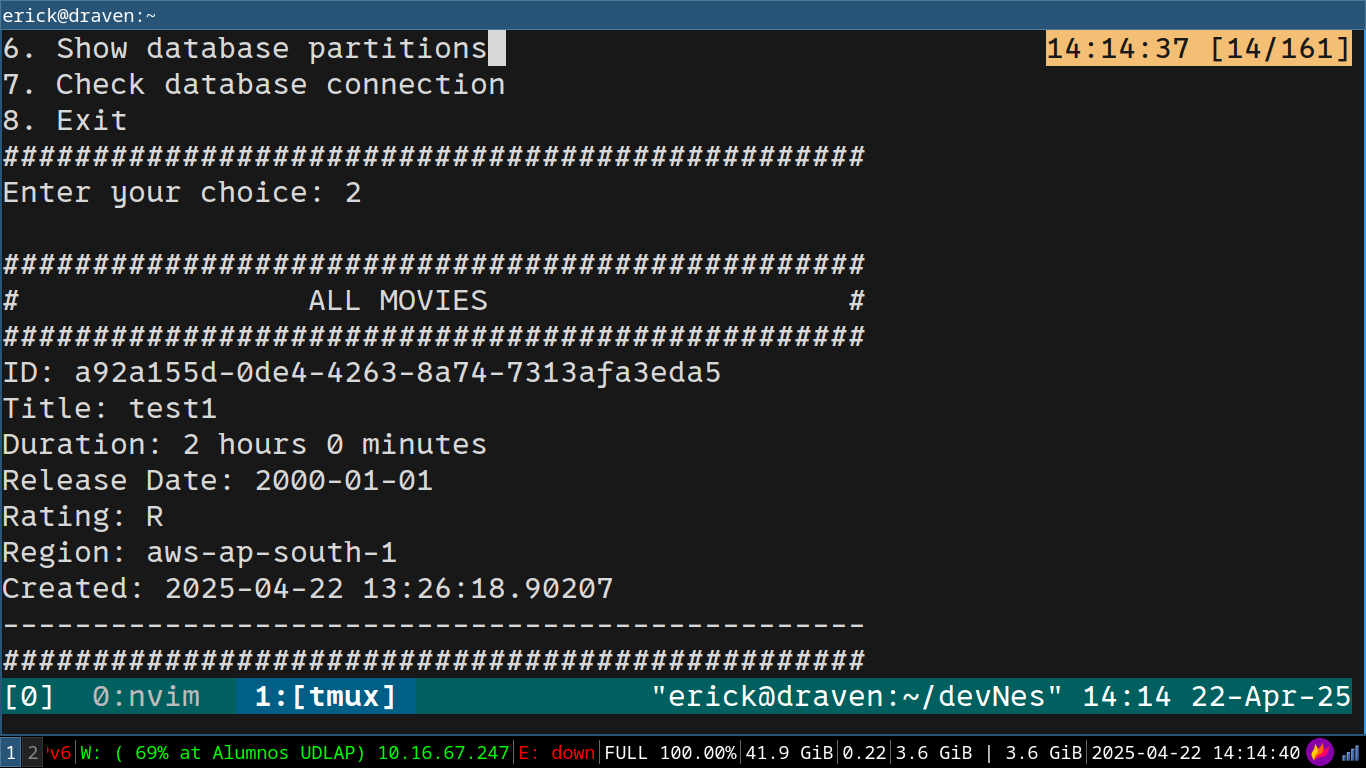
\includegraphics[width=1\textwidth]{imgs/jav2.png}
  \caption{Showing movie data}
  \label{fig:5}
\end{figure}

\begin{figure}[H]
  \centering
  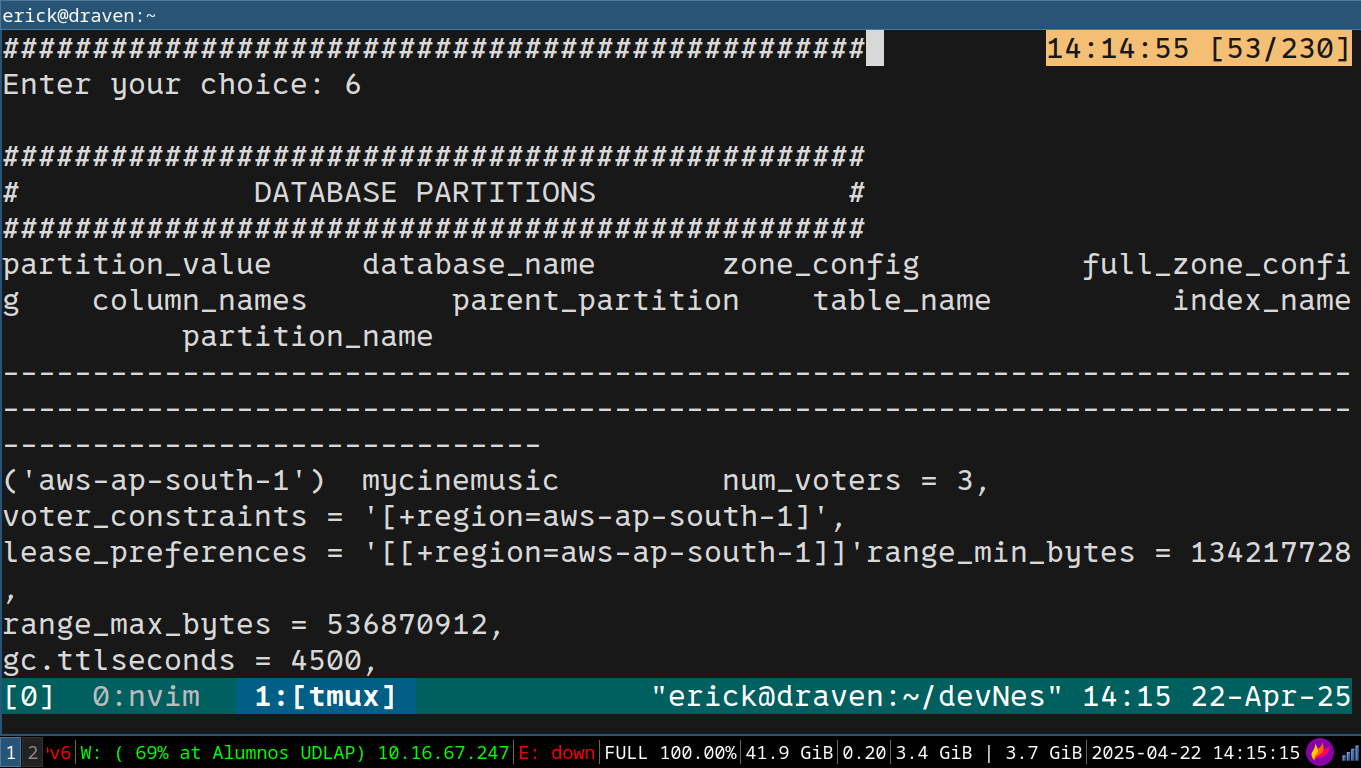
\includegraphics[width=1\textwidth]{imgs/jav3.png}
  \caption{Showing fragmentation here too}
  \label{fig:6}
\end{figure}

\section{Setting Up and Running the Software}

This section provides detailed instructions for setting up and running the distributed database application. Following these steps will allow you to experience the vertical fragmentation implementation firsthand.

\subsection{Prerequisites}

Before you begin, ensure you have the following prerequisites installed:

\begin{itemize}
  \item Java Development Kit (JDK) 21 or higher
  \item PostgreSQL JDBC Driver (version 42.7.5 or compatible)
  \item Git (for cloning the repository)
  \item Internet connection (for accessing the CockroachDB cluster)
\end{itemize}

\subsection{Environment Setup}

\subsubsection{1. Clone the Repository}

First, clone the repository to your local machine:

\begin{lstlisting}[language=bash, caption=Cloning the Repository]
git clone --recursive https://github.com/HugeErick/DistribuitedSystem.git
cd DistribuitedSystem
\end{lstlisting}

\subsubsection{2. Download the CockroachDB Root Certificate}

The application connects to a CockroachDB cluster using SSL. You need to download the root certificate to establish a secure connection.

For Unix/Linux/macOS:
\begin{lstlisting}[language=bash, caption=Downloading Certificate on Unix/Linux/macOS]
curl --create-dirs -o $HOME/.postgresql/root.crt 'https://cockroachlabs.cloud/clusters/690e5a03-c6aa-48d5-82b8-60ec652e68f7/cert'
\end{lstlisting}

For Windows:
\begin{lstlisting}[language=bash, caption=Downloading Certificate on Windows]
# Create the directory if it doesn't exist
mkdir -p "$env:APPDATA\postgresql"

# Download the certificate
curl -o "$env:APPDATA\postgresql\root.crt" "https://cockroachlabs.cloud/clusters/690e5a03-c6aa-48d5-82b8-60ec652e68f7/cert"
\end{lstlisting}

\subsubsection{3. Set Up the Environment Variable}

The application requires a JDBC connection string to connect to the CockroachDB cluster. Set up the environment variable as follows:

For Unix/Linux/macOS:
\begin{lstlisting}[language=bash, caption=Setting Environment Variable on Unix/Linux/macOS]
export JDBC_DATABASE_URL="jdbc:postgresql://free-tier14.aws-us-east-1.cockroachlabs.cloud:26257/defaultdb?sslmode=verify-full&user=<username>&password=<password>"
\end{lstlisting}

For Windows (Command Prompt):
\begin{lstlisting}[language=bash, caption=Setting Environment Variable on Windows (CMD)]
set JDBC_DATABASE_URL=jdbc:postgresql://free-tier14.aws-us-east-1.cockroachlabs.cloud:26257/defaultdb?sslmode=verify-full&user=<username>&password=<password>
\end{lstlisting}

For Windows (PowerShell):
\begin{lstlisting}[language=bash, caption=Setting Environment Variable on Windows (PowerShell)]
$env:JDBC_DATABASE_URL="jdbc:postgresql://free-tier14.aws-us-east-1.cockroachlabs.cloud:26257/defaultdb?sslmode=verify-full&user=<username>&password=<password>"
\end{lstlisting}

Replace \texttt{<username>} and \texttt{<password>} with the actual database credentials.

\subsection{Compiling and Running the Application}

\subsubsection{1. Compile the Java Code}

Compile the Java source files using the following command:

For Unix/Linux/macOS:
\begin{lstlisting}[language=bash, caption=Compiling on Unix/Linux/macOS]
javac -d bin -cp postgresql-42.7.5.jar src/*.java
\end{lstlisting}

For Windows:
\begin{lstlisting}[language=bash, caption=Compiling on Windows]
javac -d bin -cp postgresql-42.7.5.jar src\*.java
\end{lstlisting}

\subsubsection{2. Run the Application}

Run the compiled application using the following command:

For Unix/Linux/macOS:
\begin{lstlisting}[language=bash, caption=Running on Unix/Linux/macOS]
java -cp bin:postgresql-42.7.5.jar Main
\end{lstlisting}

For Windows:
\begin{lstlisting}[language=bash, caption=Running on Windows]
java -cp bin;postgresql-42.7.5.jar Main
\end{lstlisting}

\subsection{Using the Application}

Once the application is running, you will see the main menu with the following options:

\begin{enumerate}
  \item Add a new movie
  \item View all movies
  \item View movie by ID
  \item Update a movie
  \item Delete a movie
  \item Show database partitions
  \item Check database connection
  \item Exit
\end{enumerate}

\subsubsection{Adding a Movie}

To add a new movie:
\begin{enumerate}
  \item Select option 1 from the main menu
  \item Enter the movie title
  \item Enter the duration (format: 2h 30m or 150m)
  \item Enter the release date (format: YYYY-MM-DD)
  \item Enter the rating (e.g., PG-13, R)
  \item Select a region from the available options
\end{enumerate}

\subsubsection{Viewing Vertical Fragmentation}

To observe the vertical fragmentation in action:
\begin{enumerate}
  \item Select option 6 from the main menu
  \item The application will display the partition information, showing how data is distributed across different regions
\end{enumerate}

\subsection{Troubleshooting Common Issues}

\subsubsection{Connection Issues}

If the application fails to connect to the database:
\begin{enumerate}
  \item Verify that the \texttt{JDBC\_DATABASE\_URL} environment variable is correctly set
  \item Check that the username and password in the connection string are correct
  \item Ensure you have internet connectivity
  \item Verify that the PostgreSQL JDBC driver is in the classpath
\end{enumerate}

\subsubsection{ClassNotFoundException}

If you encounter a \texttt{ClassNotFoundException} for \texttt{org.postgresql.Driver}:
\begin{enumerate}
  \item Ensure the PostgreSQL JDBC driver JAR file is in the same directory as your application
  \item Verify that the JAR file is correctly included in the classpath when running the application
\end{enumerate}

\section{Conclusions}
The design of the MyCineMusic database addresses the fundamental needs for managing multimedia data related to music and cinema. It includes both the conceptual and relational schemas and provides a clear interface for interacting with the system through a defined set of queries.

Our practical implementation using Java and CockroachDB demonstrates how vertical fragmentation can be achieved in a distributed database environment. By partitioning data by region, we can optimize data locality, improve performance, and ensure regulatory compliance.

The implementation showcases several key concepts in distributed database systems:
\begin{itemize}
  \item Vertical fragmentation through region-based partitioning
  \item ACID-compliant distributed transactions
  \item SQL interface for interacting with distributed data
  \item Visualization of data distribution across regions
\end{itemize}

This approach provides a solid foundation for building scalable, resilient, and globally distributed database applications.

\begin{thebibliography}{9}
  \bibitem{cockroachlabs}
  CockroachDB. (2023). Multi-Region Capabilities. CockroachDB Documentation. Retrieved April 22, 2025, from \url{https://www.cockroachlabs.com/docs/stable/multiregion-overview.html}
  
  \bibitem{geekforgeeks}
  GeeksforGeeks. (2018, June 11). Distributed Database System. Retrieved from \url{https://www.geeksforgeeks.org/distributed-database-system/}
  
  \bibitem{mongodb}
  MongoDB. (2023). What is a Distributed Database? MongoDB Documentation. Retrieved April 22, 2025, from \url{https://www.mongodb.com/resources/basics/databases/distributed-database}
  
  \bibitem{ozsu}
  Özsu, M. T., \& Valduriez, P. (2020). Principles of Distributed Database Systems (4th ed.). Springer.
  
  \bibitem{date}
  Date, C. J. (2003). An Introduction to Database Systems (8th ed.). Addison-Wesley.
\end{thebibliography}
\end{document}
